\documentclass{article}
\usepackage{graphicx} % Required for inserting images
\usepackage{amsmath}
\usepackage{booktabs}
\usepackage{rotating}

\usepackage[utf8]{inputenc}
\usepackage[english]{babel}

\title{Additional Analysis for Optimizer Comparison}
\author{anna.shundeeva}
\date{May 2026}

\begin{document}

\maketitle

\section{Identified Mistakes}

\begin{figure}[ht]
    \centering
    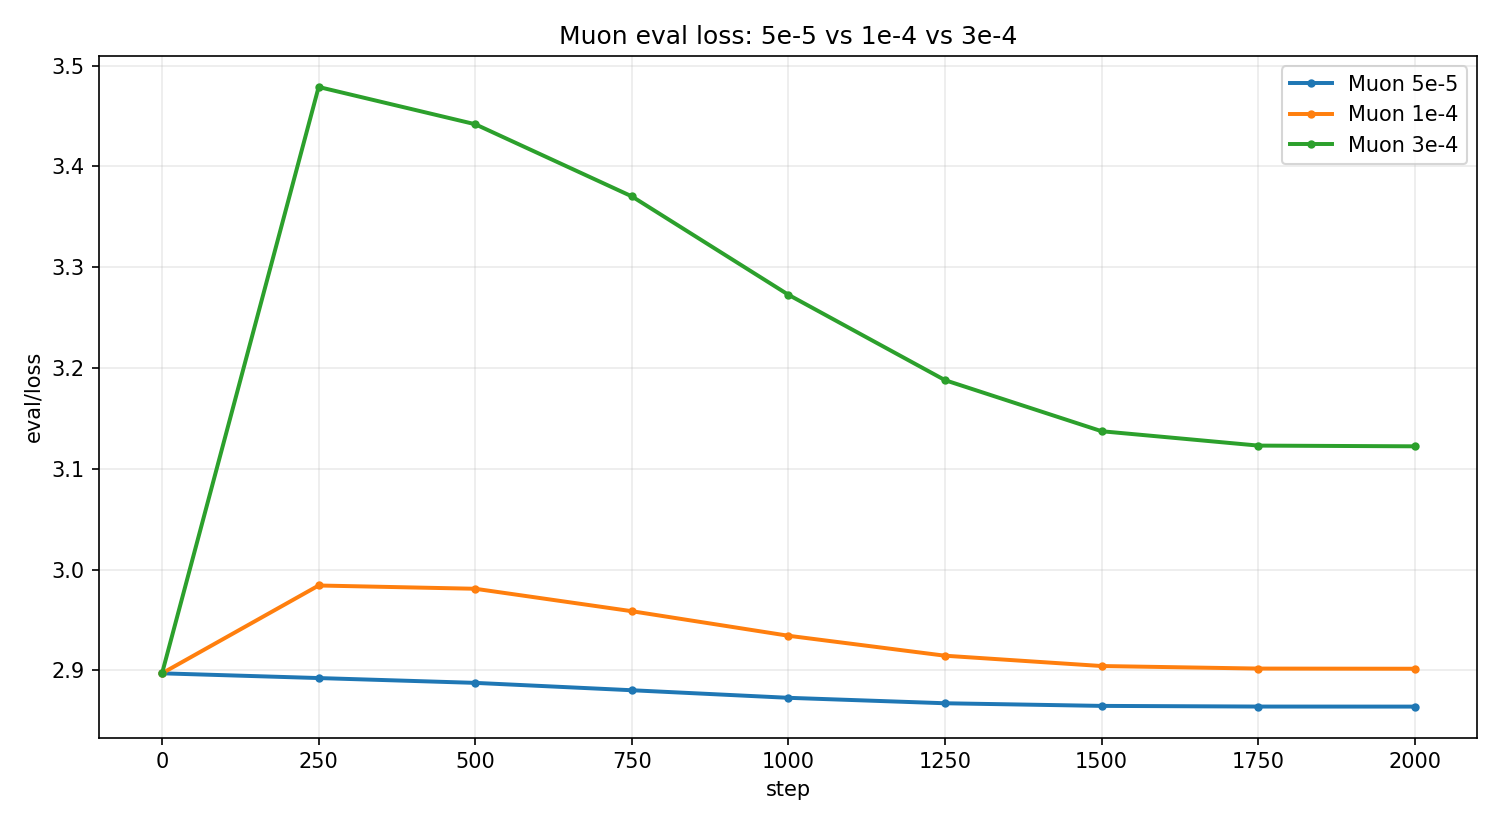
\includegraphics[width=1\textwidth]{images/eval_loss_muon_diff_lr.png}
    \caption{Validation loss for Muon with different learning rate values. Step 0 corresponds to the evaluation of the base pretrained model before fine-tuning.}
    \label{fig:muon-lr-sensitivity}
\end{figure}

One of the main mistakes in the original hyperparameter grid was choosing an overly aggressive learning rate for Muon. The paper from which the Muon implementation was taken considers both pretraining and supervised fine-tuning. In the pretraining setting, the authors use a learning rate on the order of $10^{-4}$ at a late stage of training, whereas for supervised fine-tuning the learning rate is chosen to be substantially smaller. Based on this, and also on the assumption that a somewhat larger learning rate could be acceptable both for a smaller model and for non-supervised fine-tuning, the following grid was chosen in the experiment:

$$
\{5 \cdot 10^{-5}, 10^{-4}, 3 \cdot 10^{-4}\}.
$$

However, the results show that the upper part of this grid was too large for this fine-tuning scenario. As can be seen from the plot, fine-tuning remains stable at $5 \cdot 10^{-5}$: the validation loss gradually decreases relative to the baseline. At $10^{-4}$, the model first becomes worse and only partially returns to its initial level by the end of training. At $3 \cdot 10^{-4}$, the validation loss sharply increases during the first 250 steps, after which the model does not recover to the baseline quality within 2000 steps.

This behavior can be explained by the fact that in the Muon implementation used in this experiment, the nominal learning rate is additionally scaled for matrix parameters depending on the matrix shape:

$$
\texttt{adjusted\_lr} = \texttt{adjust\_lr\_for\_muon}(\texttt{lr}, \texttt{p.shape}).
$$

$$
\texttt{adjusted\_ratio} = 0.2 * \texttt{math.sqrt(max(A, B))}.
$$

In this experiment, the largest Qwen2.5-0.5B matrices optimized with Muon were MLP matrices of size $4864 \times 896$. For such matrices, the scaling factor is approximately

$$
0.2 \sqrt{4864} \approx 13.95.
$$

Therefore, the nominal learning rate turns into the following effective learning rate for these matrices:

$$
5 \cdot 10^{-5} \rightarrow 7.0 \cdot 10^{-4},
$$

$$
10^{-4} \rightarrow 1.4 \cdot 10^{-3},
$$

$$
3 \cdot 10^{-4} \rightarrow 4.2 \cdot 10^{-3}.
$$

Thus, the value $3 \cdot 10^{-4}$ in fact led to very large updates of the MLP matrices, which is especially risky for fine-tuning. The model parameters are already reasonably well tuned, and improvement happens as careful adaptation; a strong restructuring of the weights can move the model out of the current local minimum, after which most of training is spent searching for a new one, which may not even reach the quality of the previous solution. At $3 \cdot 10^{-4}$, this is exactly what happened: the weights became destabilized, validation loss sharply increased already at the first evaluation point, and further training only partially compensated for the damage.

Therefore, the poor result of Muon at $3 \cdot 10^{-4}$ should not be interpreted as a general failure of the optimizer. A more accurate interpretation is that the original learning rate grid was poorly adapted to short full fine-tuning of an already pretrained model.

\section{Computational Costs}

\begin{table}[ht]
\centering
\resizebox{\textwidth}{!}{%
\begin{tabular}{llccc}
\toprule
Optimizer & LR & Training time (sec) & Max memory (MB) & Avg harness score \\
\midrule
AdamW & $5 \cdot 10^{-5}$ & 5156.04 & 8803.88 & 0.5407 \\
Muon & $5 \cdot 10^{-5}$ & 5402.74 & 8122.34 & 0.5424 \\
Combined & $5 \cdot 10^{-5}$ & 5276.73 & 8464.02 & 0.5425 \\
\bottomrule
\end{tabular}%
}
\caption{Computational costs at the same learning rate.}
\label{tab:same-lr-resource-efficiency}
\end{table}

Since the forward and backward passes for all three runs are performed on the same model and with the same training hyperparameters, it is reasonable to assume that the difference in step time is mainly related to the optimizer step and the accompanying operations. This is consistent with the structure of Muon: unlike AdamW, it performs an additional matrix normalization of the update through Newton--Schulz iterations, which makes the optimizer step itself more expensive.

$$
t_{step} =
t_{forward} +
t_{backward} +
t_{optimizer} +
t_{other}.
$$

Consider the total training time for the runs with learning rate $5 \cdot 10^{-5}$:

$$
T_{\text{AdamW}} \approx 5156 \text{ sec},
$$

$$
T_{\text{Muon}} \approx 5403 \text{ sec},
$$

$$
T_{\text{Combined}} \approx 5277 \text{ sec},
$$

then the average time of one training step can be estimated as

$$
t^{step}_{\text{AdamW}} \approx \frac{5156}{2000} = 2.58 \text{ sec/step},
$$

$$
t^{step}_{\text{Muon}} \approx \frac{5403}{2000} = 2.70 \text{ sec/step},
$$

$$
t^{step}_{\text{Combined}} \approx \frac{5277}{2000} = 2.64 \text{ sec/step}.
$$

The observed difference between AdamW and Muon is

$$
2.70 - 2.58 = 0.12 \text{ sec/step},
$$

which means that Muon was approximately

$$
\frac{2.70}{2.58} \approx 1.047
$$

or $4.7\%$ slower in wall-clock time per step.

The combined optimizer occupies an intermediate position, receiving half of the additional cost of Muon:

$$
2.64 = 2.58 + \frac{2.70 - 2.58}{2}.
$$

In terms of memory, a similar intermediate picture is observed, but in the opposite direction: Muon uses less GPU memory than AdamW, and Combined is almost exactly in the middle between them.

$$
8803.88 - 8122.34 = 681.54 \text{ MB}.
$$

$$
\frac{8803.88 + 8122.34}{2} = 8463.11 \text{ MB}.
$$

The actually measured value for Combined was $8464.02 \text{ MB}$, so the deviation from the average is only

$$
8464.02 - 8463.11 = 0.91 \text{ MB}.
$$

This agrees well with the architecture of the combined optimizer: in 12 out of 24 layers, part of its matrix parameters is updated with Muon, while the other half uses only AdamW for all parameters. Therefore, the combined optimizer preserves roughly half of the memory benefit that full Muon provides compared with AdamW, and receives roughly half of the additional time cost per step.

\section{Comparison of AdamW, Muon, and the Combined Optimizer}

\subsection{Validation loss dynamics}
Despite the unsuccessful choice of the upper part of the learning rate grid for Muon, one set of experiments is suitable for a minimal comparison of AdamW, Muon, and the combined optimizer. At learning rate $5 \cdot 10^{-5}$, all three training variants remain stable and make it possible to compare not only final metric values, but also the dynamics of validation loss.

\begin{figure}[ht]
    \centering
    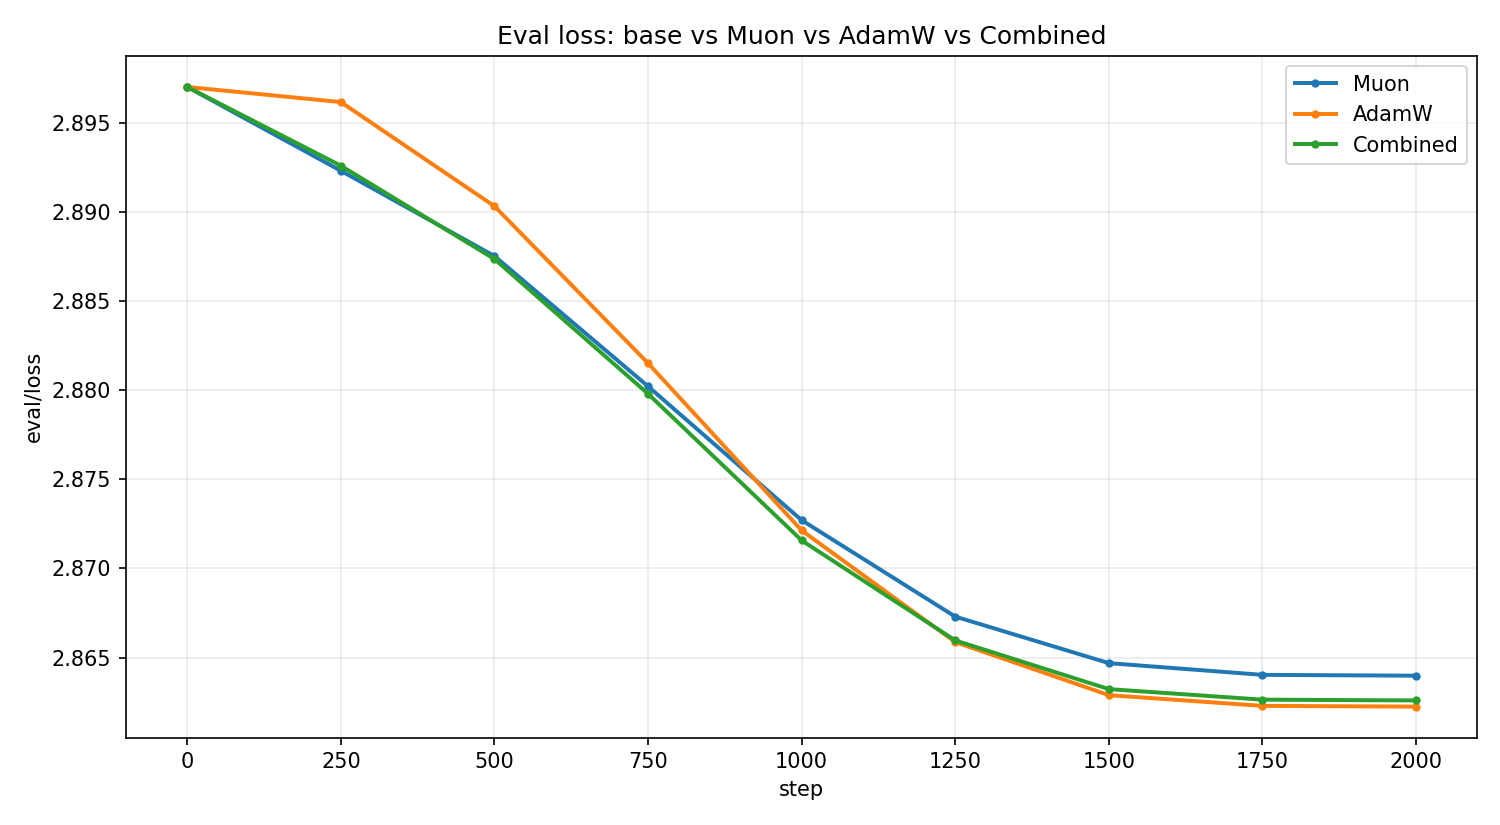
\includegraphics[width=1\textwidth]{images/eval_loss_muon_adamw_combined_with_base.png}
    \caption{Validation loss for AdamW, Muon, and the combined optimizer at learning rate $5 \cdot 10^{-5}$. Step 0 corresponds to the evaluation of the base pretrained model before fine-tuning.}
    \label{fig:adamw-muon-combined-loss}
\end{figure}

In the initial part of training, Muon decreases validation loss faster than AdamW: after the first 0--500 steps, its loss value is noticeably lower than AdamW's. This fits well with the architectural differences: by updating a matrix as a whole object, Muon can make more substantial changes at once and perform more effective updates during the early stage of fine-tuning.

However, this advantage is preserved only at the beginning of training. After approximately 1000--1500 steps, the Muon curve noticeably slows down and approaches a plateau. AdamW, on the other hand, initially decreases loss more slowly, but then continues to improve validation loss more steadily and reaches a slightly better value by the end of training. This is consistent with the idea of a more careful element-wise optimizer that accumulates its own adaptive statistics for each parameter.

The combined optimizer shows intermediate but substantively interesting behavior. At the beginning, its curve is close to Muon: validation loss decreases quickly during the first steps. At the same time, closer to the end of training, it does not reach a plateau as early as pure Muon and becomes closer to AdamW. This may be explained by the fact that at the beginning, the main adaptation is performed by the matrices in the first half of the layers, which are updated with Muon and provide faster initial progress, while the parameters of the second half of the model, trained with AdamW, preserve fine-grained element-wise adaptation during later steps.

This idea, however, is not obvious and requires additional evidence. A suitable experiment would be to repeat training while logging parameter changes and to compare their magnitude in the Muon and full-AdamW halves throughout training.

\subsection{Evaluation results}

The selected evaluation benchmarks can be divided into several semantic groups,
each testing different capabilities of the model.

\begin{table}[ht]
\centering
\begin{tabular}{llcccc}
\toprule
& & \multicolumn{2}{c}{ARC Challenge} & \multicolumn{2}{c}{ARC Easy} \\
\cmidrule(lr){3-4} \cmidrule(lr){5-6}
Optimizer & LR
& \texttt{acc} & \texttt{acc\_norm}
& \texttt{acc} & \texttt{acc\_norm} \\
\midrule
Base Qwen2.5-0.5B & -- & 0.2892 & 0.3200 & 0.6423 & 0.5816 \\
\midrule
AdamW    & $5 \cdot 10^{-5}$ & 0.2884 & 0.3225 & 0.6557 & 0.6330 \\
Muon     & $5 \cdot 10^{-5}$ & 0.2944 & 0.3268 & 0.6587 & 0.6296 \\
Combined & $5 \cdot 10^{-5}$ & 0.2884 & 0.3251 & 0.6599 & 0.6296 \\
\bottomrule
\end{tabular}
\caption{ARC Easy and ARC Challenge results at learning rate $5 \cdot 10^{-5}$.}
\label{tab:arc-results}
\end{table}

ARC Easy and ARC Challenge evaluate the model's ability to answer school-level
science questions from different domains, including chemistry, physics, biology,
and related fields. ARC Easy contains simpler and more direct questions, whereas
ARC Challenge is the harder part of the benchmark and more often requires not
only factual knowledge but also additional reasoning.

As shown in Table~\ref{tab:arc-results}, all optimizers noticeably improve the
results on ARC Easy, the facts for which can be found in OpenWebText-100k, a 
collection of random texts from the Internet, in one form or another almost 
directly.

For ARC Challenge, the picture is less clear. However, on ARC Challenge, 
which requires more reasoning, the results are much more unstable and close to the 
uncertainty of a single run. If Qwen2.5-0.5B can improve on this task using this 
dataset at all (for example, AdamW with $3 \cdot 10^{-5}$ shows a hopefull result),
then the current 2000 steps and the selected learning rate are poorly suited
for this setting.

\begin{table}[ht]
\centering
\begin{tabular}{llcccc}
\toprule
& & \multicolumn{2}{c}{HellaSwag} & \multicolumn{2}{c}{PIQA} \\
\cmidrule(lr){3-4} \cmidrule(lr){5-6}
Optimizer & LR
& \texttt{acc} & \texttt{acc\_norm}
& \texttt{acc} & \texttt{acc\_norm} \\
\midrule
Base Qwen2.5-0.5B & -- & 0.4059 & 0.5210 & 0.7046 & 0.6970 \\
\midrule
AdamW    & $5 \cdot 10^{-5}$ & 0.3984 & 0.5025 & 0.6959 & 0.6921 \\
Muon     & $5 \cdot 10^{-5}$ & 0.3989 & 0.5032 & 0.6970 & 0.6942 \\
Combined & $5 \cdot 10^{-5}$ & 0.3978 & 0.5015 & 0.6986 & 0.6921 \\
\bottomrule
\end{tabular}
\caption{HellaSwag and PIQA results at learning rate $5 \cdot 10^{-5}$.}
\label{tab:hellaswag-piqa-results}
\end{table}

HellaSwag and PIQA both evaluate aspects of commonsense reasoning. HellaSwag
tests whether the model can choose the most plausible continuation of an
everyday scenario, whereas PIQA is more closely related to physical commonsense
and practical interactions with objects.

On OpenWebText-100k, these metrics can improve only indirectly: through the
general presence of everyday situations in web text and through a possible
improvement in the model's overall ability to generalize. Given the limitations
of the small Qwen2.5-0.5B model and the short fine-tuning run, this is unlikely. 
As shown in Table~\ref{tab:hellaswag-piqa-results}, it does not appear in this 
experiment. All optimizers slightly degrade the result. A likely interpretation 
is that the relatively active weight shift caused by fine-tuning at learning rate 
$5 \cdot 10^{-5}$ partially disrupts some of the base model's existing zero-shot 
capabilities.

\begin{table}[ht]
\centering
\begin{tabular}{llc}
\toprule
Optimizer & LR & WinoGrande \\
\midrule
Base Qwen2.5-0.5B & -- & 0.5627 \\
\midrule
AdamW    & $5 \cdot 10^{-5}$ & 0.5533 \\
Muon     & $5 \cdot 10^{-5}$ & 0.5580 \\
Combined & $5 \cdot 10^{-5}$ & 0.5643 \\
\bottomrule
\end{tabular}
\caption{WinoGrande results at learning rate $5 \cdot 10^{-5}$.}
\label{tab:winogrande-results}
\end{table}

WinoGrande stands somewhat apart from the other evaluation benchmarks. This task
tests the model's ability to resolve ambiguity within a short textual context and
choose the more plausible option using commonsense reasoning. At first glance,
OpenWebText-100k may seem suitable for this type of task. However, the structure of WinoGrande requires the model to
interpret relations within the written context rather than simply memorize a
specific type of text.

As shown in Table~\ref{tab:winogrande-results}, AdamW and Muon degrade the result
relative to the base model. This can be interpreted as another indication that
learning rate $5 \cdot 10^{-5}$ may be too large in this fine-tuning setup to
preserve the model's more delicate zero-shot capabilities.

The Combined optimizer performs unexpectedly well and slightly exceeds the
baseline. However, the absolute difference is too small to be interpreted as a
reliable advantage from a single run. Therefore, this result is not sufficient to
conclude that any architectural property of the Combined optimizer is genuinely
better suited for WinoGrande-like tasks.

Overall, on this set of evaluation metrics, the fine-tuned models behave in a
way that is more strongly determined by the relationship between the benchmark
type, the fine-tuning dataset, and the relatively aggressive learning rate than
by the optimizer type itself. In addition, having only one run for each optimizer
does not allow us to reliably separate random variation in a particular run from
general trends.

\section{Additional Conclusions}

Although one Muon step was slightly more expensive, its validation loss decreased faster than AdamW's at the early steps. Therefore, for evaluating practical efficiency, it is important to compare not only the time of one step, but also the time required to reach a given quality level.

If a certain target loss is reached after $S_{\text{AdamW}}$ AdamW steps and after $S_{\text{Muon}}$ Muon steps, then Muon is more beneficial in wall-clock time under the condition

$$
S_{\text{Muon}} \cdot t^{step}_{\text{Muon}}
<
S_{\text{AdamW}} \cdot t^{step}_{\text{AdamW}}.
$$

Taking into account the measured step times:

$$
S_{\text{Muon}} \cdot 2.70
<
S_{\text{AdamW}} \cdot 2.58.
$$

Therefore,

$$
S_{\text{Muon}}
<
0.956 \cdot S_{\text{AdamW}}.
$$

That is, Muon must reach the same quality with at least about $4.4\%$ fewer steps in order to compensate for the more expensive optimizer step. In the early part of training, this condition may hold: Muon decreases validation loss faster during the first approximately 500 steps.

The behavior of the combined optimizer should also be noted separately. It uses less memory and less wall-clock time than full Muon, but in the early steps it shows very similar validation loss dynamics. Apparently, applying Muon only to half of the model layers is sufficient for fast initial adaptation; it is also possible that the effect will persist if an even smaller fraction of layers is used or if some matrices are additionally excluded.

However, this conclusion requires separate verification. In the current experiment, only one parameter-splitting strategy was tested, so it cannot be claimed that the chosen Muon/AdamW proportion is optimal. A more accurate conclusion is that the combined optimizer looks like a promising direction for further research: it partially preserves Muon's early dynamics, while having a lower cost and coming closer to AdamW's stability.

It should also be mentioned that all the conclusions and calculations described above were made based on a single run. Despite their general consistency with other work on the topic and with theoretical expectations, they cannot be considered sufficiently reliable.

\end{document}
